\documentclass[10pt,twoside]{article}
\usepackage[utf8]{inputenc}
\usepackage{natbib}
\usepackage{graphicx}
\usepackage{booktabs}
\usepackage{adjustbox}
\usepackage[table,xcdraw]{xcolor}
\usepackage{amsmath}
\usepackage[]{todonotes}
\usepackage{fancyhdr}
\usepackage{multirow}

% Idioma
\usepackage[english]{babel}

\usepackage[none]{hyphenat}

\usepackage[Alg.]{algorithm}
\usepackage{algpseudocode}

\newcommand{\ignore}[1]{}


\title{Constructive Sweep-Based Algorithm for Heterogeneous Cumulative Capacitated Vehicle Routing Problem}
\author{\emph{David Plazas Escudero}\\
\vspace{0.3cm}
\small{\tt{dplazas@eafit.edu.co}}\\
Departamento de Ciencias Matemáticas\\
Escuela de Ciencias\\
Universidad EAFIT\\
Medellín -- Colombia}
\date{}

\usepackage{anysize}
\marginsize{3cm}{2cm}{2cm}{3cm}

% Configurar encabezado y pie de página
\pagestyle{fancy}
\lfoot[\date{\today}]{\date{\today}}
\rfoot[\thepage]{\thepage}
\cfoot[]{}
\rhead[Plazas (2019)]{Constructive Algorithm for Heterogeneous Cumulative Capacitated Vehicle Routing Problem}
\lhead[]{}

\fancypagestyle{firststyle}
{
   \fancyhf{}
   \fancyfoot[R]{Last updated: August 19, 2019}
}

\sloppy



\begin{document}

\maketitle

\thispagestyle{firststyle}

% \begin{abstract}
% Buenas
% \vspace{0.2cm}\\
% %
% \noindent \textbf{Keywords:}
% Heuristic, constructive algorithm, vehicle routing problem, heterogeneous-fleet.
% \end{abstract}

\section{Algorithm Description}\label{sec_intro}

The algorithm presented in this work is inspired on the well-known sweep algorithm, proposed by \cite{gillett1974heuristic}; this procedure swipes the nodes by its polar phase relative to the deposit and adds them to routes until the capacity constrain is exceeded. The original algorithm is intended to give solution to an homogeneous-fleet vehicle routing problem (VRP). Another important reference for the ideas of this paper is presented by \cite{suthikarnnarunai2008sweep}, where the author makes a suggestion for the heterogeneous-fleet VRP. The procedure presented in this work is based on both ideas and creates an algorithm that gives a suitable solution, minimizing the number of nodes unassigned.

The suggestion from \cite{suthikarnnarunai2008sweep} is to take the largest capacity vehicle and apply the standard sweep approach and take the resulting routes with the maximum amount of nodes visited; the here presented algorithm takes this idea and changes this criterion to: take the resulting routes with maximum used capacity, mixing this with the ``parent'' node idea (explained in next sections) the algorithm was developed.

\subsection{General Steps}
The algorithm takes as input a set of types of vehicles with their respective capacity, relative speed factor and the number of available vehicles of each type; and a set of nodes with their spatial coordinates and demands.

\begin{enumerate}
  \item For each node, calculate the relative coordinates from the depot: Let $(x_0,\,y_0)$ be the spatial coordinates of the depot, the relative coordinates of the $i$-th node are:\[(\tilde{x}_i, \tilde{y}_i):=(x_i-x_0,y_i-y_0).\]
  \item Calculate the associated phase $\varphi_i\in[-\pi,\,\pi]$ for each node with
  \[\varphi_i := \arctan\left(\dfrac{\tilde{y}_i}{\tilde{x}_i}\right).\]
  \item Sort the resulting phases increasingly.
  \item Sort the vehicles by capacity, decreasingly.
  \item For each type of vehicle $m$, starting from the one with higher capacity, create routes using each vehicle $k$, starting from the node with maximum demand; the starting node on each iteration shall be called ``parent'' node. The algorithm appends nodes to the parent route sweeping through the sorted phases (starting counterclockwise) until the capacity of the current vehicle is exceeded. When sweeping the phases, if the next node is last one (or first one) in the sorted phase array, the algorithm returns to the parent node and starts to append in the opposite direction from the previous one (clockwise). Once the routes have been created, select the $N_k$ routes with highest demand and permanently assign the nodes in these routes with the associated vehicle $k$.
  \item Once this process has been completed for all vehicles, check for unassigned nodes and attempt to assign them to existing routes; this step is intended to minimize the amount of unassigned nodes, even though it can deteriorate the objective function.
  \item Calculate the value of the objective function $z$, iterating through the created routes and through each node, adding the time of all the route starting from the current node; the time is calculated as the euclidean distance from the current node to the next node and multiplying it by the relative speed factor; then multiply by the demand (coefficient in the objective function).
\end{enumerate}

\subsection{Sweeping Step}
This section is devoted to make a better explanation of the procedure already described in step 5 of the preceding section. For example, in the following figure, the phase ordering is depicted:
\begin{figure}[H]
    \centering
    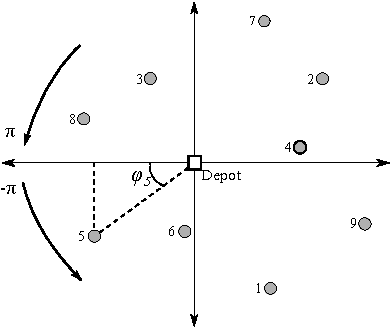
\includegraphics[scale=1.4]{figs/drawing.pdf}
    \caption{Phase Ordering.}
    \label{fig:phase_order}
\end{figure}
In this particular case, the phase ordering would be: [5, 6, 1, 9, 4, 2, 7, 3, 8]. Let us assume that the node with higher demand is number 3, thus 3 is the parent node. The algorithm would search in counterclockwise direction for nodes: in this case, the next one is 8; but there would not be a next node to sweep after 8, since the array ends there; therefore, the algorithm switches to clockwise direction starting from 3 again, adding 7 and so forth. 

\section{Results}
This paper is not intended to propose an efficient and well-thought lower bound for the HCCVRP. The lower bound used here is a quite simple solution but the lower bound is not good. The lower bound is obtained assuming an ``infinite'' amount of vehicles and assigning a node per vehicle, creating routes visiting only one node. It is trivial that this lower bound is beyond the optimal solution to the problem here treated. Let $z_{lb}$ be the found lower bound, the formula for calculating the relative distance to the lower bound is
\[\text{LB-Comparison}=\dfrac{z-z_{lb}}{z_{lb}}\times100.\%\]

The relative distance to the LB of the obtained solution, as well as the execution time, are presented in the following table:
\begin{table}[H]
\centering
\begin{tabular}{ccccc}
\hline
\textbf{Instance} & \textbf{Nodes} & \textbf{LB Comparison (\%)} & \textbf{A. E. T. (s)} & \textbf{T. T. (s)} \\ \hline
1                 & 50             & 615.06                      & 0.0009971             & 0.0019944          \\
2                 & 50             & 640.03                      & 0.0009971             & 0.0039897          \\
3                 & 50             & 696.11                      & 0.0019932             & 0.0049853          \\
4                 & 75             & 411.74                      & 0.0019958             & 0.0039897          \\
5                 & 75             & 412.95                      & 0.0019922             & 0.0049860          \\
6                 & 75             & 426.51                      & 0.0029938             & 0.0049863          \\
7                 & 100            & 775.27                      & 0.0029933             & 0.0059845          \\
8                 & 100            & 782.82                      & 0.0029929             & 0.0059835          \\
9                 & 100            & 755.65                      & 0.0029931             & 0.0059841          \\
10                & 150            & 652.55                      & 0.0059521             & 0.0099738          \\
11                & 150            & 729.45                      & 0.0059848             & 0.0099747          \\
12                & 150            & 655.37                      & 0.0049825             & 0.0089757          \\
13                & 199            & 961.49                      & 0.0139620             & 0.0189488          \\
14                & 199            & 497.72                      & 0.0119676             & 0.0159561          \\
15                & 199            & 467.59                      & 0.0129933             & 0.0169566          \\
16                & 120            & 1153.37                     & 0.0039892             & 0.0059993          \\
17                & 120            & 631.15                      & 0.0039887             & 0.0069639          \\
18                & 120            & 636.36                      & 0.0039887             & 0.0079805          \\
19                & 100            & 527.22                      & 0.0019941             & 0.0049848          \\
20                & 100            & 596.37                      & 0.0020254             & 0.0040212          \\
21                & 100            & 623.61                      & 0.0019681             & 0.0039575          \\ \hline
\end{tabular}
\caption{Results for each instance}
\label{tab:results}
\end{table}

Table \ref{tab:results} shows the percentage lower-bound comparison for each instance, as well as the algorithm execution time (A. E. T.) in seconds and the total time (T. T.) also in seconds. The T. T. takes into consideration the reading process for each data set, the calculation of the objective function and writing the output data. These results were obtained in a home desktop PC with a 4.2GHz Intel Core i7-7700k.

\subsection{Comparison with other Heuristics}
Given that the used lower bound cannot provide enough information, the results will be compared with other constructive algorithms proposed by colleagues. The first one (A1), proposed by Juan S. Cárdenas, and the second one, proposed by Mateo Restrepo, are both adaptations of the well-known savings algorithm proposed by \cite{clarke1964scheduling}. The objective function value was compared with:
\[\text{z-Comparison}=\dfrac{z-z_{i}}{z_{i}}\times100\%\]
where $z_i$ for $i=1,\,2$ are the objective function value obtained with their heuristics, and $z$ the one with the algorithm presented in this work. The results are presented in the following table:
\begin{table}[H]
\centering
\begin{tabular}{cccc}
\hline
\textbf{Instance} & \textbf{Nodes} & \textbf{A1 (\%)} & \textbf{A2(\%)} \\ \hline
1                 & 50             & 21.38            & -11.48          \\
2                 & 50             & 31.89            & -22.79          \\
3                 & 50             & 56.79            & -24.23          \\
4                 & 75             & 33.43            & -5.78           \\
5                 & 75             & 42.68            & -8.92           \\
6                 & 75             & 38.99            & -9.90           \\
7                 & 100            & 82.96            & -17.35          \\
8                 & 100            & 63.33            & -21.29          \\
9                 & 100            & 59.64            & -38.50          \\
10                & 150            & 72.01            & -23.19          \\
11                & 150            & 86.12            & 0.55            \\
12                & 150            & 48.26            & -24.74          \\
13                & 199            & 51.58            & -6.59           \\
14                & 199            & 42.98            & -4.43           \\
15                & 199            & 63.31            & 0.29            \\
16                & 120            & 109.96           & 4.81            \\
17                & 120            & 107.43           & -12.63          \\
18                & 120            & 69.07            & -16.04          \\
19                & 100            & 91.67            & -19.39          \\
20                & 100            & 64.24            & -10.52          \\
21                & 100            & 74.18            & -10.71          \\ \hline
\end{tabular}
\caption{Results for different heuristics for each instance.}
\label{tab:otherRes}
\end{table}
\section{Conclusion}
This works presents an heuristic constructive algorithm for the HCCVRP. The results obtained show that the algorithm is really fast, even for ``large'' problems; on the other hand, the algorithm cannot be properly validated using lower-bounds. Nevertheless, the algorithm was compared with other constructive algorithms proposed by colleagues and the objective functions here obtained are relatively close to theirs, in some cases better. The resulting algorithm, given its fast execution time, can be used as initial solution for more elaborated procedures.



%%%%%%%%%%%%%%%%%%%%%%%%%%%%%%%%%%%%%%%%%%%%%%%%%%%%%%%%%%%%%%%%%%%%%%%%%%%%%%%%%%%%%%%%%%%%
\section*{Acknowledgements}
%%%%%%%%%%%%%%%%%%%%%%%%%%%%%%%%%%%%%%%%%%%%%%%%%%%%%%%%%%%%%%%%%%%%%%%%%%%%%%%%%%%%%%%%%%%%
The author wishes to thank his colleague Juan S. Cárdenas for his valuable discussion regarding the implementation of the presented algorithm; and both Juan S. Cárdenas and Mateo Restrepo for allowing the author to use their results as reference.


{\small
\bibliographystyle{authordate1}

\bibliography{bibs}}


\end{document}
